\documentclass[tikz,border=10pt]{standalone}
\usepackage{tikz}
\usepackage{listings}
\usetikzlibrary{arrows.meta, positioning}
\lstset{language=C, basicstyle=\ttfamily}

\begin{document}

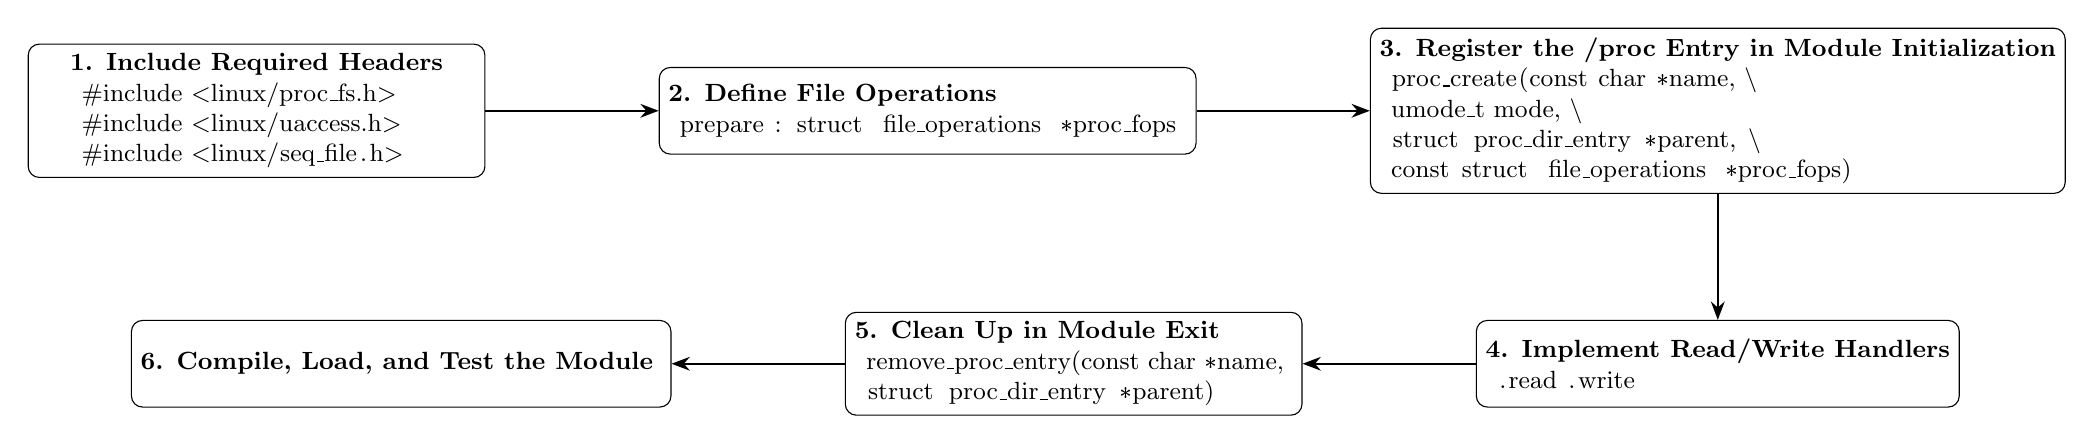
\begin{tikzpicture}[
    box/.style={
        draw,
        rounded corners,
        minimum width=5.8cm,
        minimum height=1.1cm,
        align=left,
        font=\small
    },
    arrow/.style={
        ->,
        thick,
        >=Stealth
    },
    node distance=1.6cm and 2.2cm
]

% First row: left to right
\node[box] (step1) {
    \textbf{1. Include Required Headers} \\
    \lstinline| #include <linux/proc_fs.h> | \\
    \lstinline| #include <linux/uaccess.h> | \\
    \lstinline| #include <linux/seq_file.h> |
};

\node[box,right=of step1] (step2) {
    \textbf{2. Define File Operations} \\
    \lstinline| prepare : struct file_operations *proc_fops |
};

\node[box,right=of step2] (step3) {
    \textbf{3. Register the /proc Entry in Module Initialization} \\
    \lstinline| proc_create(const char *name, \ | \\
    \lstinline| umode_t mode, \ | \\
    \lstinline| struct proc_dir_entry *parent, \  | \\
    \lstinline| const struct file_operations *proc_fops) |

};

% Second row: right to left
\node[box,below=of step3] (step4) {
    \textbf{4. Implement Read/Write Handlers} \\
    \lstinline| .read .write |
};

\node[box,left=of step4] (step5) {
    \textbf{5. Clean Up in Module Exit} \\
    \lstinline| remove_proc_entry(const char *name, | \\
    \lstinline| struct proc_dir_entry *parent) |
};

\node[box,left=of step5] (step6) {
    \textbf{6. Compile, Load, and Test the Module}
};

% Arrows
\draw[arrow] (step1) -- (step2);
\draw[arrow] (step2) -- (step3);
\draw[arrow] (step3) -- (step4);
\draw[arrow] (step4) -- (step5);
\draw[arrow] (step5) -- (step6);

\end{tikzpicture}

\end{document}
